\chapter{The Ford Challenge} 
In this chapter, the ford competition that is the basis for this report, is introduced. Before introducing the ford challenge, a short overview of other online machine learning competitions is given. As part of introducing the ford competition, the kaggle.com website that hosted the ford competition is presented, and the data set used in the ford competition is described in detail. But as metioned the chapter starts with a short overview of other online machine learning competitions.

\section{Other online machine learning competitions}
To get a little perspective on the ford challenge, this section gives a short review of some past and present online machine learning competitions.

\subsection{Netflix Prize}
One of the most talked about competitions, may very well be the Netflix Prize. The Netflix competition was launched on October 2, 2006 and the aim of the competition was to predict how users would grade new movies, based on a large dataset of previous grades. Why did the Netflix Prize gather a lot of attention? First of all the grand prize was \$1M, which is a lot of money. And secondly the dataset was huge, consisting of 100,480,507 ratings given by 480,189 users, leaving room for a lot of interesting new techniques to be tested. \par 
When the Netflix Prize was awarded on September 18, 2009, 5169 different teams had submitted at least one entry to the competition. The winning team consisted of three different teams, that at one point decided to team-up and compete as a join-team.\par 
Netflix originally wished to follow up the Netflix Prize, with another competition but decided to dismiss the idea, due to a lawsuit regarding privacy concerns related to the first Netflix Prize. \footnote{The section about The Netflix Prize is based on \citet{wiki:netflix_prize} and \citet{netflix_leaderboard}}

\subsection{KDD Cup}
Although the Netflix Prize gather a lot attention, it wasn't the first online machine learning competition. An example of an earlier competition, is the KDD Cup. The KDD Cup is a competition that is held every year, and that started back in 1997. The subject changes every year, and can be anything from mining purchase data from an online store, to computer aided detection of breast cancer (the 2000 and 2008 competitions respectively).\par
This year the KDD Cup is held in coorporation with Yahoo! Labs and the task is to predict user ratings of musical items (both tracks, albums, artists and genres). One note worthy detail about the 2011 KDD Cup is the huge data set, containing over 300 million ratings of more than 600,000 distinct items. \footnote{Read more about the KDD Cup history at \citet{kdd_cup_center}. For more info about the 2011 competition see \citet{kdd_cup_2011}}

\subsection{And many others}
The Netflix Prize and the KDD Cup are just two examples of online machine learning competitions. Many others exists, such as
\begin{itemize}
    \item \emph{The Hearst Challenge 2011} - Every year The Hearst Corporation hosts a machine learning competition. This year the task is to data mine the history of 1.8 million emails sent to subscribers of Hearst's publications, and then predict who will open emails in the future. \\
        Read more at \url{http://www.hearstchallenge.com}
    \item \emph{The Reclab Prize} - RichRelevance is a company that specializes in online product recommendation. They offer a \$1M prize for the team that first improves their product recommendation algorithm by 10\%. \\
        Read more at \url{http://www.overstockreclabprize.com}
    \item \emph{The Heritage Health Prize} - 
\end{itemize}
Since almost all the machine learning competition websites, needs the same functionality, websites that specializes in hosting machine learning competitions has appeared. One example of a website that provides a hosting platform for machine learning competitions is the kaggle.com website, who hosts The Ford Challenge.

\section{Kaggle.com and The Ford Challenge}
As already mentioned, kaggle.com hosts machine learning competitions for universities and corporations. The first competition hosted by kaggle.com was started in April 2010, and since then a total of 18 competitions have been held. Every competition at kaggle.com has some background information, links to the data sets, a submission system and a forum, as seen in figure \ref{fig:fordchallenge_frontpage}. \par

\begin{figure}[tbhHp]
    \centering
        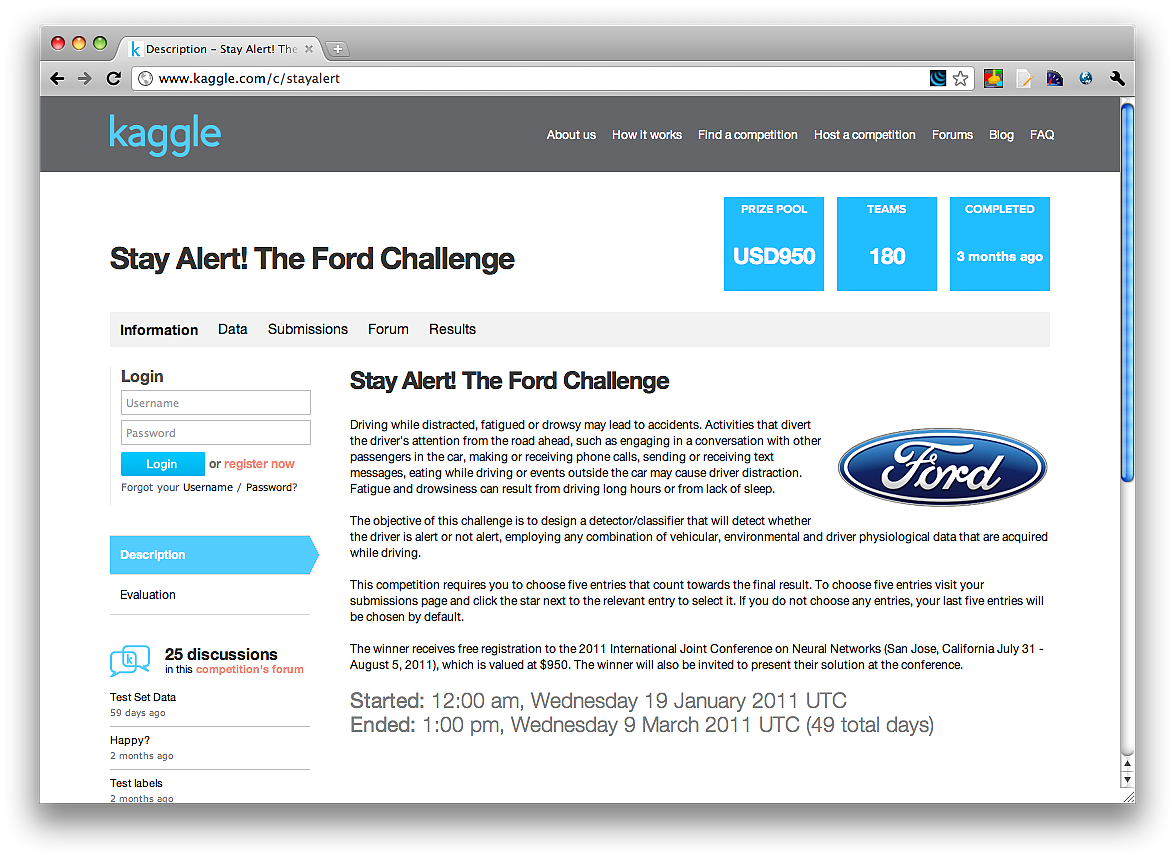
\includegraphics[width=.9\textwidth]{media/fordchallenge_frontpage.png}
    \caption{The Ford Challenge frontpage at the kaggle.com website}
    \label{fig:fordchallenge_frontpage}
\end{figure}

The Ford Challenge began on January 19, 2011. The task was to create a classifier that is able to detect when a driver is about to get distracted while driving. The dataset that Ford made available for the competition consisted of measurements of 30 different features, measured on drivers along with a binary feature (IsAlert) that was 1 if the driver was alert and 0 otherwise. The 30 features was a mix of environmental, driver physiological and vehicular features\footnote{The dataset is explained in much more detail in the section \ref{sec:the-competition:dataset}}. Based on this dataset a classifier should predict the IsAlert feature of a distinct test dataset held by Ford. \par
One detail that made the competition slightly different than many other competitions, was that Ford would not disclose any information about what the different features represented\footnote{see forum replies from the Ford spokesperson \citep{kaggle_forum_266,kaggle_forum_317}}. The official reason was that \citep{kaggle_forum_268_reply_2}
\begin{quote}
    ``We like to encourage the participants to pursue classification without preconceived notions based on prior knowledge of the subject, focusing on variables which lead them (based on their own experiments) to better classification."
\end{quote}
Doubts about the true motive behind the lack of details about the features, was expressed by, what later turned out to be, the winner of the competition \citep{kaggle_forum_295_reply_3} \par

The performance of the classifiers was measured by calculating the AUC (see section \ref{sec:theory:auc}) of the classifiers, on the test set. A limit of two submissions per contestant was set as a way to counteract the possibility of someone reverse-engineering the IsAlert-feature of the test dataset. This could of cause be circumvented by one person registering more than once. And this was exactly what happened. On March 9, 2011 when the competition ended, two users had achieved exactly the same AUC (six significant digits) and other contestants immediately questioned the probability of two unrelated users getting exactly the same AUC \citep{kaggle_forum_327_reply_1}. One of the two leaders (Rosanne/Shen) quickly admitted that he and his friend had indeed used two accounts to get 4 submission per day \citep{kaggle_forum_327_reply_4}, and after some discussion in the forum, the leaders were disqualified. The end result was that the user Inference in third position was declared the official winner of the competition. \par

Two weeks after the competition ended, Inference described the technique used to win the competition. This will be described in detail in chapter \ref{sec:recreating}. But before that chapter, the data set will be described in details in the next section.

\subsection{The data set}\label{sec:the-competition:dataset}
\begin{table}
    {\small\sffamily
    \begin{tabularx}{\textwidth}{ | l l l R R R R R R R R R | }
        \hline
        TrialID & ObsNum & IsAlert & P1 & $\dots$ & P8 & E1 & $\dots$ & E11 & V1 & $\dots$ & V11 \\\hline
        0 & 0 & 0 & 12.2 & $\dots$ & 1.2 & 4.3 & $\dots$ & 33 & 12 & $\dots$ & 7.34 \\
        $\vdots$ & & & & & & & & & & &$\vdots$ \\
        0 & 1200 & 1 & 11.1 & $\dots$ & 10.7 & 1.3 & $\dots$ & 21 & 8 & $\dots$ & 8.82 \\
        $\vdots$ & & & & & & & & & & &$\vdots$ \\
        510 & 1198 & 0 & 11.1 & $\dots$ & 10.7 & 1.3 & $\dots$ & 21 & 8 & $\dots$ & 8.82 \\\hline
    \end{tabularx}
    }
    \caption{Structure of the data set}
    \label{tbl:structure-of-data}
\end{table}
The dataset used to create a classfier was released on the competition website, the day the competition started. The dataset consisted of a number of trials and each trial was approximately 2 minutes of sequential data recorded every 100ms during a driving session on the road or in a driving simulator \citep{kaggle_data}. As the interval between two \mydef{rows} was 100ms, each trial consists of approximately $2\,\text{minutes}\cdot 60\,\frac{\text{secs}}{\text{minute}} \cdot 10\,\frac{\text{rows}}{\text{sec}}=1200$ rows. \par
Each row has a total of 33 data columns structured as shown in table \ref{tbl:structure-of-data}. Some details are worth noticing:
\begin{itemize}
    \item The \fn{TrialID} starts at 0 and the trials from 469 to 479 (both inclusive) are missing. The last trial has \fn{TrialID=510}. This gives a total of exactly 500 trials.
    \item The \fn{ObsNum} also starts at 0 there are not exactly 1200 observation for every trial.
    \item The total number of rows is 604,229
    \item The row number is not part of the data set, so a row is uniquely identified by the pair (\fn{TrialID}, \fn{ObsNum}).
\end{itemize}
As mentioned before no additional information about what the different features represent or what datatype (discrete, continous) they are, was disclosed by Ford. The only way to get these informations is by doing af thorough data exploration of the data set and that is what the next chapter is about.
